\documentclass{article}
\usepackage[utf8]{inputenc}
\usepackage[portuges]{babel}
\usepackage[a4paper, total={7in, 9in}]{geometry}
\usepackage{graphicx}
\usepackage{float}
\usepackage{caption}
\usepackage{fancyvrb}

\newcommand{\question}[1]{
    {\large \textbf{Q: #1}}
    \\
}

\newcommand{\titleRule}{
    \rule{\linewidth}{0.5mm} \\ [0.25cm]
}

\begin{document}

{
\center
\textsc{\Large Universidade do Minho} \\ [0.5cm]
\textsc{\Large Mestrado em Engenharia Informática} \\ [0.5cm]
\textsc{\large Tecnologia de Segurança} \\ [0.5cm]

{\LARGE \bfseries MellonFS : Userspace filesystem } \\[0.5cm]

\begin{tabular}{c}
    Miguel Miranda Quaresma \\
    A77049  \\
\end{tabular} \\[0.5cm]

\today \\[1cm]
}

\section{Introdução}
Os mecanismos de controlo de acesso são uma das partes fundamentais dos sistemas de computação atuais, desempenhando um papel fundamental ao
permitirem a utilização destes sistemas de uma forma partilhada por diversos utilizadores em simultâneo. 
Como tal, é necessário desenvolver mecanismos de controlo que permitam mediar o acesso partilhado a estes recursos, garantindo a sua integridade 
e restringindo o acesso aos utilizadores autorizados. Dada a diversidade de contextos em que é necessário a implementação destes mecanismos o 
uso de sistemas de permissões como os apresentados pelo sistema operativo Unix é inadequado dada a sua primitividade e inflexibilidade, sendo 
útil desenvolver sistemas de controlo que implementem estruturas mais complexas adaptadas ao contexto para o qual são desenvolvidos. 
O presente trabalho propõe uma possível implementação para um destes mecanismos de controlo, designado MellonFS, que, com recurso a um 
segredo/código aletório gerado \textit{on demand} e a uma lista de utilizadores autorizados, visa mediar este acesso de forma segura e conveniente.

\section{MellonFS}
O sistema proposto foi desenvolvido com uma arquitetura constituída por dois módulos distintos, que comunicam entre si: 
\begin{itemize}
    \item uma \textit{web interface}, desenvolvida em Python, responsável por iniciar a execução do \textit{daemon} e que permite ao utilizador 
    identificar-se perante o sistema e, posteriormente, introduzir os códigos de autenticação que lhe são enviados de modo a poder aceder aos 
    ficheiros pretendidos
    \item um \textit{daemon}, desenvolvido em C, que implementa o sistema de ficheiros com recurso à biblioteca libfuse sendo ainda responsável 
    por gerar um código de autenticação cada vez que é invocada a \textit{system call} \texttt{open}
\end{itemize}

\subsection{Implementação}
\subsubsection{Web Frontend}
A \textit{web fronted} foi desenvolvida com recurso à linguagem Python e à framework \textit{Flask}.
Como foi referido esta componente é responsável por iniciar o \textit{daemon} com os argumentos necessários ao seu funcionamento.
Antes de invocar o mesmo a \textit{frontend} requisita o \textit{username} ao utilizador que permitirá determinar se este se 
encontra, ou não, autorizado a aceder aos ficheiros no sistema desenvolvido. Este valor será também ele passado como argumento ao 
\textit{daemon}:
\begin{Verbatim}
args=['./bin/mellon', '../MountPoint']
...
mellon_fs = Popen(args)
\end{Verbatim}
As comunicações entre os dois processos/componentes são efetuadas com recurso a um \textit{named pipe}, que é aberto para escrita no 
\textit{frontend}:
\begin{Verbatim}
mellon_fifo = open("mellon_fifo", "w")
...
if request.method == 'POST':
    code = request.form['fa_code']
    mellon_fifo.write(code[:5])
    mellon_fifo.flush()
\end{Verbatim}
Na posse da \textit{master key}(=123456789), o \textit{frontend} permite ainda o registo de novos utilizadores,
rejeitando qualquer tentativa de registo caso o valor introduzido para a mesma seja inválido:
\begin{figure}[H]
    \centering
    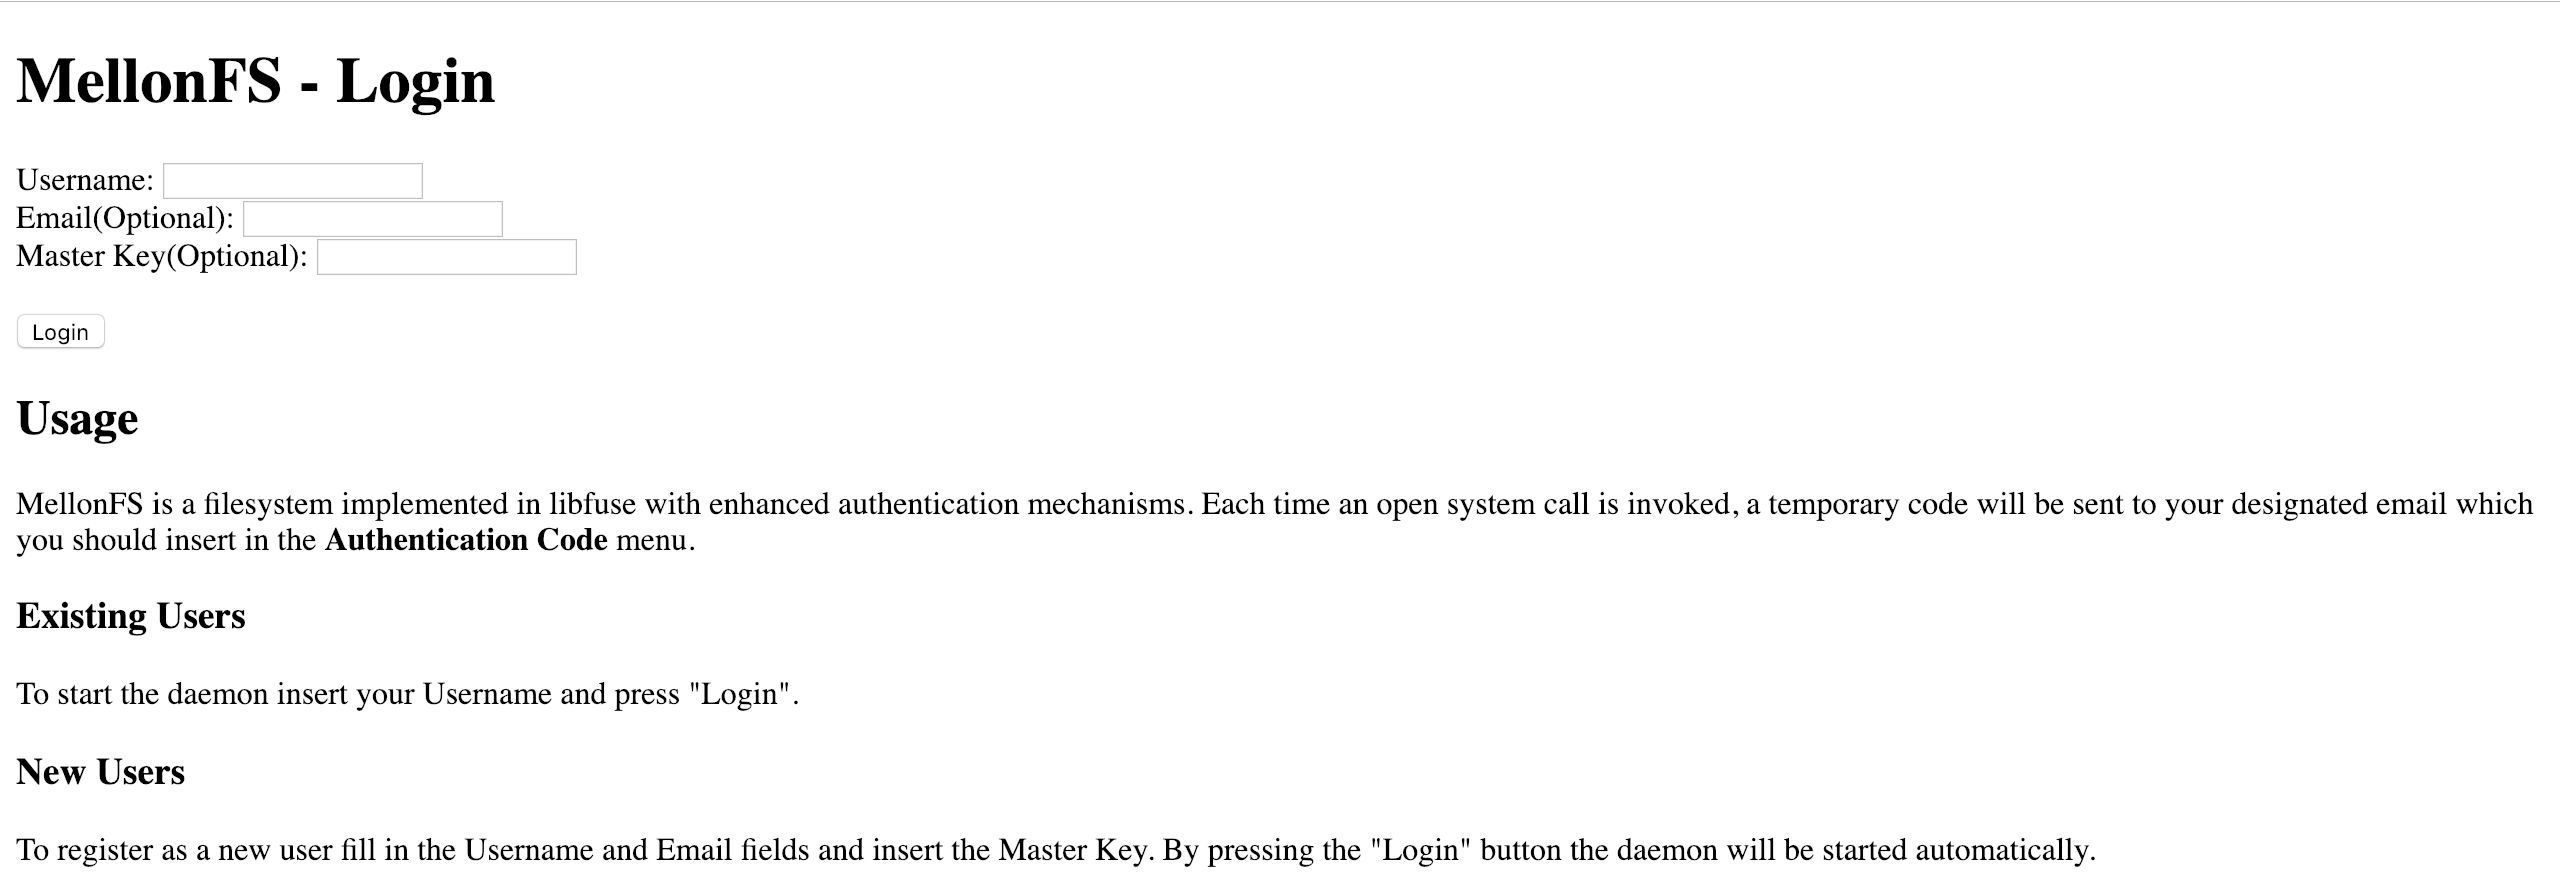
\includegraphics[width=10cm]{Pictures/Main.png}
\end{figure}
Após a identificação perante o sistema é apresentado um menu onde devem ser inseridos, quando necessário, os códigos enviados para o endereço
de email do utilizador:
\begin{figure}[H]
    \centering
    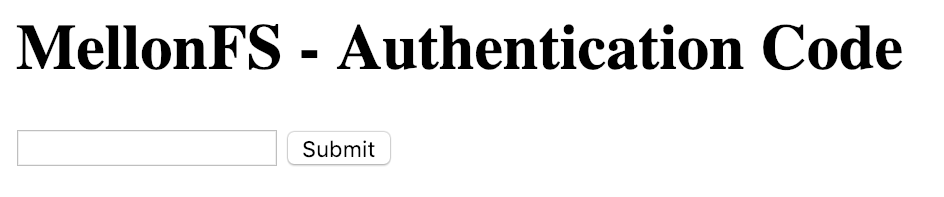
\includegraphics[width=5cm]{Pictures/Auth.png}
\end{figure}

\subsubsection{Daemon}
O segundo componente do sistema desenvolvido é invocado pelo \textit{frontend} e implementa não só o sistema de ficheiros, mas também os mecanismos
de controlo de acesso ao mesmo. 
Antes de iniciar a execução em modo \textit{daemon} este componente verifica se a identificação apresenta pelo utilizador que requisitou o acesso 
é valida e, em caso afirmativo, prossegue a execução. Adicionalmente, caso o utilizador não esteja autorizado mas tenha sido inserida a \textit{master
key} correta, o sistema efetua o registo do utilizador, prosseguindo à invocação do \textit{dameon}.
Esta verificação prévia visa garantir que o utilizador tem permissão para aceder ao sistema de ficheiros, sendo o conjunto de utilizadores nestas 
condições armazenados no ficheiro \texttt{mellon\_acl.enc} que se encontra cifrado, via AES em modo CBC, por forma a garantir a sua integridade e 
confidencialidade. Cada vez que o \textit{daemon} inicia a sua execução este ficheiro é temporariamente decifrado(e cifrado novamente) com recurso 
à função:
\begin{Verbatim}
int encrypt_decrypt(char *source, int enc_dec)
\end{Verbatim}
que invoca a ferramenta OpenSSL:
\begin{Verbatim}
#define DEC "openssl enc -aes-256-cbc -in %s -out %s -K %s -iv %s -d"
#define ENC "openssl enc -aes-256-cbc -in %s -out %s -K %s -iv %s && rm %s"
\end{Verbatim}

Adicionalmente, a cada invocação da \textit{system call} \texttt{open} que, através da API disponibilizada pela biblioteca
libfuse, envolve uma chamada à função \texttt{mellon\_open}, é requerido ao utilizador que introduza um código aleatório de 4 caractéres:
\begin{Verbatim}
getentropy(buf, sizeof(char)*4);
\end{Verbatim}
que é enviado para o endereço de correio eletrónico do utilizador, recorrendo para isso à biblioteca \texttt{libcurl}.
Este valor é depois transferido, através de um \textit{named pipe}, para o\textit{daemon}, após ter sido introduzido pelo utilizador 
no \textit{frontend}:
\begin{Verbatim}
gettimeofday(&start, NULL);
read(mellon_fifo_fd, user_code, 4);
gettimeofday(&end, NULL);
\end{Verbatim}
A autenticação terá sucesso se:
\begin{itemize}
    \item o tempo entre o envio do código e a sua introdução não exceder 45s
    \item o valor introduzido corresponder ao valor efetivamente enviado ao utilizador (\texttt{fa\_code})
\end{itemize}

\begin{Verbatim}
//Timeout if user takes more than 45 secs do input code
if(end.tv_sec - start.tv_sec < 45 && !strcmp(user_code, fa_code))
\end{Verbatim}

\subsection{Utilização}
A página inicial da aplicação inclui uma breve descrição da mesma.
A \textit{master key}(=123456789) utilizada no registo de utilizadores e na decifragem do ficheiro \texttt{mellon\_acl.enc} encontra-se
armazenada no macro \texttt{AES\_KEY} para propósitos de teste.

\subsection{Dependências}
A aplicação desenvolvida recorre às seguintes bibliotecas:
\begin{itemize}
    \item Python Frontend
    \begin{itemize}
        \item Flask
    \end{itemize}
    \item Daemon
    \begin{itemize}
        \item libfuse
        \item libcurl
        \item OpenSSL
    \end{itemize}
\end{itemize}

\section{Conclusão}
O sistema de controlo de acesso desenvolvido, apesar de funcional e eficaz, apresenta-se como uma implementação primitiva e 
com poucas considerações para diversos aspetos que o podem tornar vulnerável a diversas ameaças, visando apenas demonstrar 
uma possível solução para o problema de controlo de acesso.
Das diversas limitações apresentadas é importante realçar algumas que devem servir de ponto de partida para uma implementação mais 
robusta:
\begin{itemize}
    \item a consulta do ficheiro (cifrado) que contém os utilizadores autorizados envolve a criação de um ficheiro, ainda que temporário, 
    com a informação em formato "limpo", comprometendo a confidencialidade da mesma
    \item a comunicação via \textit{named pipes} entre as duas componentes desenvolvidas não apresenta mecanismos que garantam a sua 
    confidencialidade nem integridade permitindo que um atacante intercete a comunicação realizando um ataque conhecido como 
    \textit{Man in the Middle} 
\end{itemize}
Apesar destas limitações a implementação proposta uma base sólida para um mecanismo de controlo de acesso que vise ser conveniente para 
os seus utilizadores e eficaz na mediação que efetua.
\end{document}